\chapter{Domain Analysis}\label{chap:prelim}
To decide what to include in narrative summaries, we analyze professional Age of Empires II (AoE2) commentary using a cross-domain lens. StarCraft II (SC2) shoutcasting work \cite{dodge2018, penney2018, penney2021}\footnote{\citet{penney2021} supersedes the earlier two papers \cite{dodge2018, penney2018}; however most of our analysis predates it. We refer to \citet{penney2021} for the most detailed findings, but otherwise cite the earlier two.} provides a reusable account of what shoutcasters say and which information they draw on. Because SC2 and AoE2 are both real-time strategy (RTS) games yet differ in pace and mechanics, we examine which findings transfer to AoE2. This analysis addresses RQ4 from Chapter~\ref{chap:introduction}, explaining what reporting strategies commentators use and how these align with viewer engagement through the following sub-questions:
\begin{enumerate}[noitemsep, topsep=0pt]
  \item \textbf{RQA1:} How similar is AoE2 to StarCraft II in terms of information and commentary strategies?
  \item \textbf{RQA2:} What information and knowledge are used to commentate on match events?
  \item \textbf{RQA3:} What narrative structure is used to report on a competitive AoE2 match?
\end{enumerate}
Which content types AoE2-specific viewers actually value is validated in the preliminary viewer study (Chapter~\ref{chap:viewer-study}).

\section{Methodology}
For this we adapt the SC2 analysis approach used by \citet{dodge2018, penney2018} to AoE2 using three lenses: (1) PEAS + Information Foraging Theory (IFT) for cue-driven information access \cite{russell1995, pirolli1999}, (2) intelligibility types \cite{lim2009} for the implicit questions answered, and (3) utterance-level coding inspired by linguistic coding work \cite{metoyer2010}. Based on our findings we motivate the design of the viewer study and yield design implications for our system.

\subsection{Information Foraging \& PEAS}
Information Foraging Theory (IFT) \cite{pirolli1999} describes the location (\textit{patches}), order and routes (\textit{paths}) of information access, and the Performance, Environment, Actuators, Sensors (PEAS) framework \cite{russell1995} describes cue-driven access to information in complex interfaces. In shoutcasting, cues are often \textit{Actuator}-level events (especially battles) \cite{penney2021}; casters then draw on \textit{Environment} (e.g., unit positions) and \textit{Performance} (e.g., production downtime) information (and occasionally \textit{Sensors}, e.g., scouting) to explain consequences. We use this \textit{Actuator}--\textit{Environment}--\textit{Performance}+\textit{Sensors} (A--E--P+S) loop (the specific PEAS foraging path found by \citet{penney2021}) as a compact concept anchor and compare if this strategy transfers to AoE2, and if so, which specific information types are used for each PEAS category.

\subsection{Linguistic Coding}
Prior work uses linguistic coding to relate what casters say to what they can observe in the game. \citet{metoyer2010} introduce a co-occurrence-based (which important words are often used together) scheme for RTS explanations, and \citet{dodge2018} apply it to SC2 shoutcasts to identify frequent action/property pairings. We use this as inspiration for AoE2, focusing on recurring event types and supporting properties that our system must surface.

\subsection{Intelligibility Types}
Intelligibility types \cite{lim2009} categorize the implicit questions that explanations answer (\textit{what}, \textit{what could happen}, \textit{how to}, \textit{why did}, \textit{why didn't}); \citet{dodge2018} adapt them to shoutcasting and add a Judgment category for evaluative statements. We use the same codes for AoE2; definitions and the SC2 comparison are summarized in Table~\ref{tab:lim-coding-compare}.

\subsection{Information \& Knowledge Sources}
\label{subsec:info-sources}
Some utterances draw on information not tied to a visible patch. Because our prototype depends on what data we can access, we categorize sources, distinguishing directly observed game/overlay information from context that comes from outside the current state or from interpretation. This categorization was adapted from \citet{zheng2025}, whose survey of automated game commentary identifies similar information types used to differentiate commentary styles; we adapt their taxonomy to our AoE2 setting. We identify:

\begin{enumerate}[noitemsep, topsep=0pt]
  \item \textbf{Descriptive Information:} Directly observed game state and events (e.g., movements, battles, production, upgrades, vision/states), often available from game data and PEAS patches with minimal processing. \textit{Example:} Blue is advancing to the Castle Age; Red has 30 Archers grouped at the north side.

  \item \textbf{Background Information:} Historical facts about players/teams and prior encounters (short-term and long-term), used for prediction or entertainment; long-term sources are often external databases while short-term sources are typically caster memory. \textit{Example:} This player won the last three matches against his opponent; he is known for aggressive strategies on this map.

  \item \textbf{Domain Knowledge:} Mechanics, strategies, and meta-game trends used to provide context and explain significance; this changes over time and often requires human interpretation or is inferred from game data. \textit{Example:} The Mayans have a strong early economy due to their cheaper Archers; Fast Castle is a common strategy on open maps.

  \item \textbf{Analytical Knowledge:} Higher-level inferences derived by combining descriptive sources (e.g., strategic decisions, economic status, skill), typically requiring interpretation and additional processing. \textit{Example:} Blue is ahead in economy but behind in military, so he will need to close his defenses; Red is likely preparing for a counter-attack based on his unit composition.

  \item \textbf{Experiential Knowledge:} Personal experiences or insider knowledge from casters' interactions and play, often used during lulls or to predict tendencies; outside the scope of this research. \textit{Example:} I've played against him before, and he loves sneaking villagers.
\end{enumerate}

These types align with play-by-play vs.\ color roles: play-by-play centers on descriptive information and domain knowledge, while color draws more on analytical, background, and experiential content \cite{kempecook2019, li2020, lewandowski2012}. We distinguish \textit{Information} (factual/observable) from \textit{Knowledge} (requires understanding/experience). We use \textit{Descriptive} for directly observed state/events (game data) and group \textit{Background}, \textit{Domain}, \textit{Analytical}, and \textit{Experiential} under \textit{Contextual information}; when tied to a focal event we call it \textit{Supporting information}, that can be used to \textit{enrich} the commentary.

\section{AoE2 Adaptation}
With the theoretical lenses established, we apply them to AoE2 in two steps: (1) identifying the game-specific events and states that CaptureAge data makes available for commentary, mapped to PEAS; and (2) defining the coding scheme. Rather than constructing a word-level co-occurrence matrix like \citet{metoyer2010}, which is time-intensive and more suited for projects where text analysis takes a more central role, we instead code each utterance with a \textit{Commentary Category} and, where applicable, a \textit{Subtype}, mapped to Information Sources to understand the relationship between the utterance and the underlying information. This captures narrative structure with less overhead while still producing a comparable picture of what casters say and why.

Both Commentary Categories and Subtypes were derived inductively from an initial coding pass of the primary shoutcast (T90 \& Nili). This is appropriate for an exploratory study: the goal is not to validate a fixed scheme but to identify the recurring patterns that can ground the prototype design.

\textbf{Commentary Categories} describe the \textit{narrative purpose} of an utterance: what communicative role it plays (e.g., describing an event, predicting strategy, updating game state). \textbf{Subtypes} further specify the \textit{topic} within a category, what specific event or state is being described (e.g., a Battle, an Age-up, Scouting). A single utterance receives one Commentary Category and, if applicable, one Subtype. Table~\ref{tab:communication-intents-descriptions} defines all Commentary Categories; Table~\ref{tab:captureage-states} lists Subtypes and their PEAS mapping.

\subsection{Information Patches}
First, we categorize the patches available for AoE2 in the CaptureAge Preview version used in our analysis (Figure~\ref{img:captureage-preview}; Table~\ref{tab:captureage-patches}), to provide a comprehensive overview of what information is regularly available to the caster. Additional tables can be found in Appendix \ref{appendix:domain-analysis-supplementary-tables}.

\begin{table}[htbp]
  \caption{Commentary Categories: inductively derived high-level coding scheme for utterance narrative purpose. Each utterance receives exactly one category.}
  \centering
  \setlength{\tabcolsep}{3pt}
  \renewcommand{\arraystretch}{1.5}
  \begin{tabularx}{\textwidth}{@{}>{\raggedright\arraybackslash}p{3.5cm}>{\raggedright\arraybackslash}p{12cm}@{}}
    \toprule
    \textbf{Comm.\ Category}  & \textbf{Description} \\
    \midrule
    Event Description      & Describing current events in the game. \\
    Strategy Discussion    & Discussing strategies and tactics employed by players, usually based on current events. \\
    Strategy Prediction    & Predicting future strategies and tactics based on current events and player behavior, either long-term or short-term. \\
    State Update           & An update about the state of the game, not directly describing an ongoing event but used as contextual information. \\
    Civilization Analysis  & Summarizing, explaining or contextualizing civilization mechanics and bonuses, used as introduction or to contextualize ongoing events. \\
    Historical Account     & Historical information relevant to the current game match, players, civilizations, or strategies. \\
    Game Discussion        & Discussing game mechanics and metagame (currently popular strategies). \\
    Off-Topic              & Content not related to the current match (or series). \\
    Player Analysis        & Discussing player trivia, including playstyles and recurring strategies. \\
    Map Analysis           & The (current) state of the map, including resource locations and player positions. \\
    Technical Issues       & Noticing bugs in the game, and commenting on them. \\
    Recap                  & Evaluating what happened in the game so far, summarizing key events and player actions. \\
    Skill Discussion       & A discussion about a player's ability to do certain things, such as micro-management and quick-walling. \\
    Joke                   & A joke to entertain the audience. \\
    Match Introduction     & Introduction of the players and their civilizations. \\
    \bottomrule
  \end{tabularx}
  \label{tab:communication-intents-descriptions}
\end{table}

\begin{figure}[htbp]
  \centering
  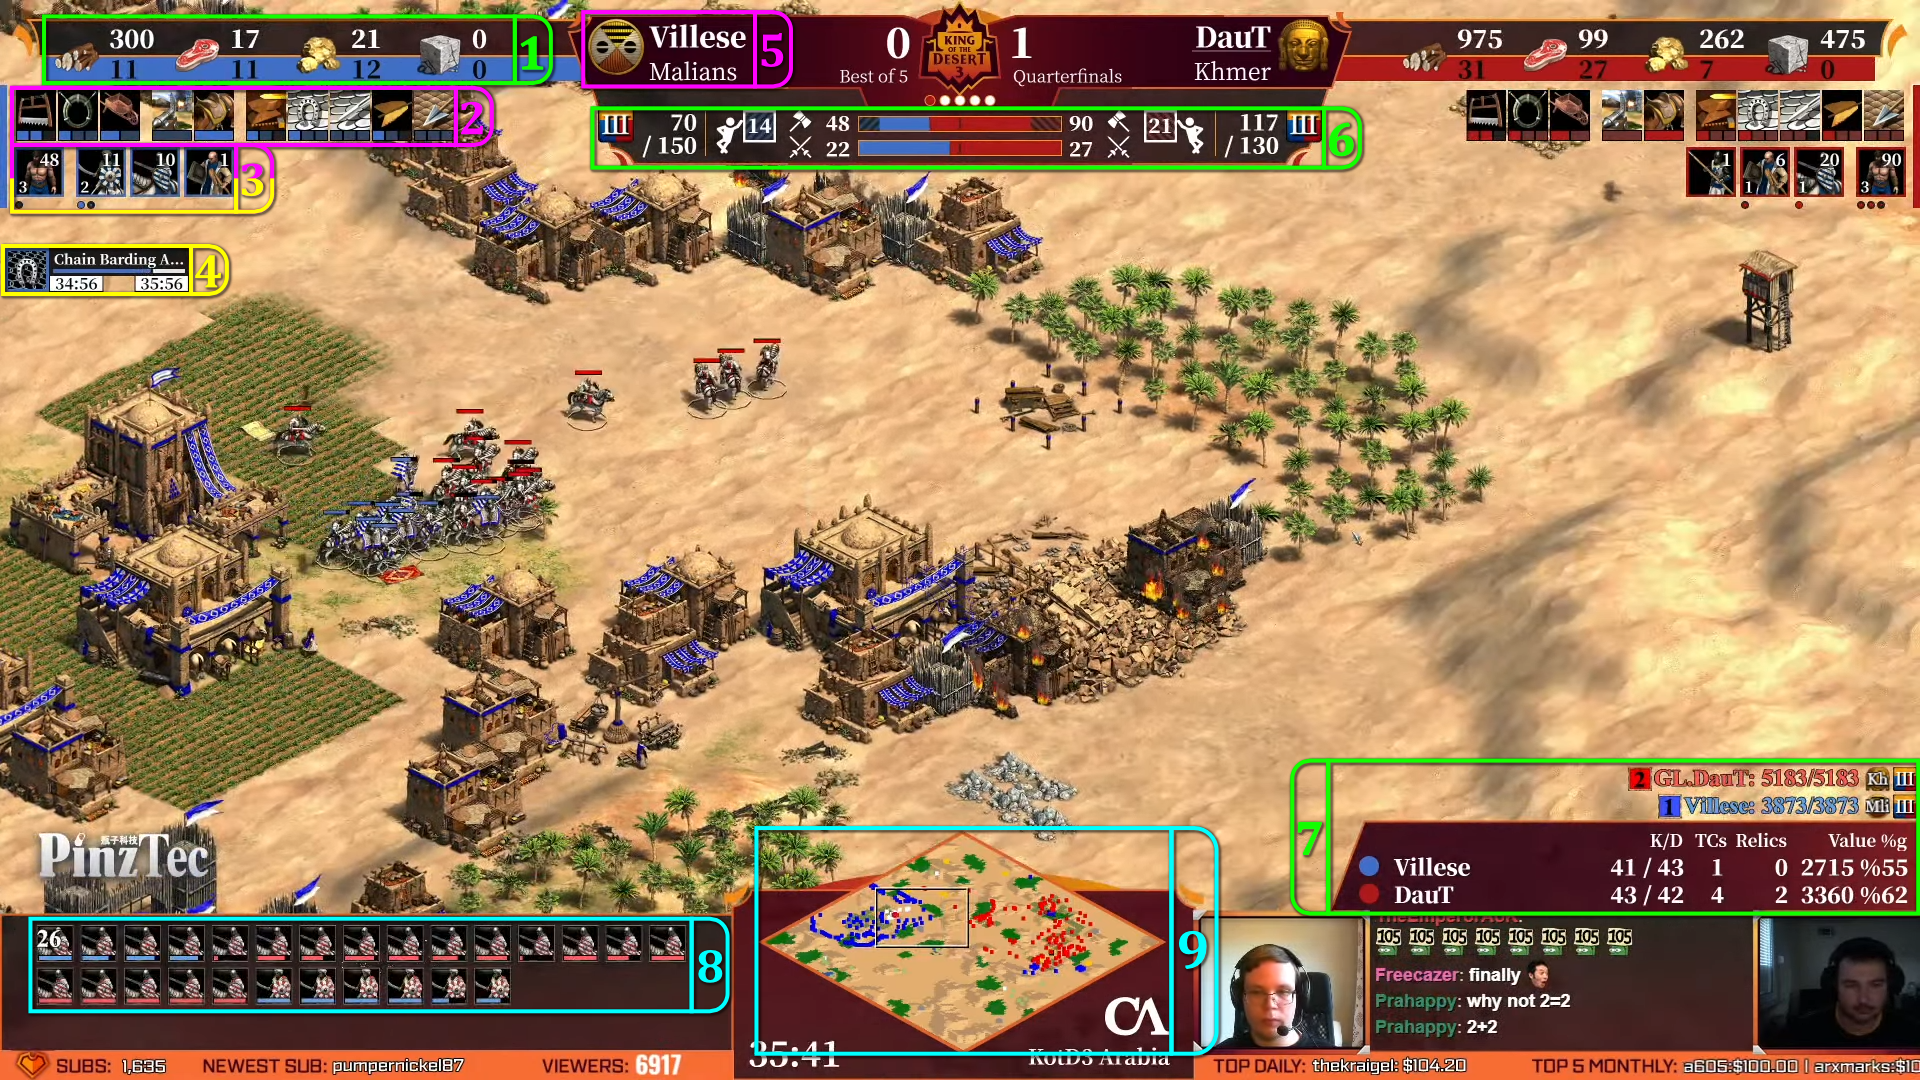
\includegraphics[width=\textwidth, height=0.9\textheight, keepaspectratio]{assets/captureage-screenshot-patches.png}
  \caption{An overview image of the CaptureAge Preview interface and its patches; see Table~\ref{tab:captureage-patches} for a description of each patch.}
  \label{img:captureage-preview}
\end{figure}
\FloatBarrier

\begin{table}[htbp]
  \centering
  \setlength{\tabcolsep}{4pt}
  \renewcommand{\arraystretch}{1.5}
  % m{} column for vertical centering, wider first col to accommodate rotated text safely
  % Use p{} instead of m{} so multirow controls the total block height cleanly
  \caption{PEAS-based patches in the CaptureAge Preview overlay. Numbers refer to Figure~\ref{img:captureage-preview}. World is intentionally added as a patch for its dual role as Environment and Actuator information, and left with no number because it is not explicitly labeled in the UI.}
  \begin{tabularx}{\textwidth}{@{}>{\centering\arraybackslash}p{0.9cm}>{\centering\arraybackslash}p{0.6cm}X X@{}}
    \toprule
    \textbf{PEAS} & \textbf{\#} & \textbf{Patch Name} \\ \midrule
    \multirow[c]{3}{0.25cm}[-1.8em]{\rotatebox[origin=c]{90}{\shortstack{Performance}}} & 1 & \textbf{Resources}: A tab showing the current amount of each resource in the player's stockpile, and the number of villagers gathering each resource. \\
    & 6 & \textbf{Key Stats Comparison}: Active age technology, total population, idle villagers, total workers, and number of military units. \\
    & 7 & \textbf{Stats Comparison}: Units killed and lost, active Town Centers, collected Relics, army value (incl. gold composition percentage). \\
    \midrule
    \multirow[c]{4}{0.25cm}[-1.5em]{\rotatebox[origin=c]{90}{\shortstack{Environment}}} & 2 & \textbf{Key Technology Status}: Status indicators for a subset of impactful technologies. \\
    & 5 & \textbf{Player Name \& Civilization}: Identifies each player and chosen civilization. \\
    & 3 & \textbf{Units (Standing)}: Number of each unit type currently deployed (top-right of each icon).\\
    & -- & \textbf{World}: All entities and terrain in the current camera view plus world overlays (entity health, building production progress). In our analysis, its main use as Environment for commentating is showing the state of the game world. \\
    \midrule
    \multirow[c]{3}{0.25cm}[-1.2em]{\rotatebox[origin=c]{90}{\shortstack{Actuators}}} & 3 & \textbf{Units (Training)}: Units currently in production (bottom-left) with progress indicators (dots). \\
    & 4 & \textbf{Technologies}: Progress toward technologies being researched. \\
    & -- & \textbf{World}: All entities and terrain in the current camera view plus world overlays (entity health, building production progress). In our analysis, its main use as Actuator for commentating is showing player actions. \\
    \midrule
    \multirow[c]{2}{0.25cm}[-1.25em]{\rotatebox[origin=c]{90}{\shortstack{Sensors}}} & 8 & \textbf{Unit Selection}: Currently selected units and their health for tactical comparison. \\
    & 9 & \textbf{Minimap}: Zoomed-out map overview for rapid spatial navigation. \\
    & -- & \textbf{Fog of War Toggle}: (Hidden control) See player's visible areas (active vision) and explored (seen, but no active vision)\\
    \bottomrule
  \end{tabularx}
  \label{tab:captureage-patches}
\end{table}

\clearpage

CaptureAge offers patches analogous to the SC2 overlay, but with persistent displays (few popups) and a more player-grouped layout. This supports both within-player interpretation (e.g., what an economy suggests about strategy) and between-player comparison (e.g., who is ahead).

Because most information is visible at all times in this CaptureAge version, we do not reconstruct explicit information-foraging paths as \citet{dodge2018} did from overlay transitions. Instead, we code utterances into Commentary Categories and Subtypes and map these to PEAS types, producing a comparable characterisation of what information supports different narrative moves.

Subtypes further specify the topic within each category. Table~\ref{tab:captureage-states} lists the Subtypes derived from the primary coding pass and their PEAS mapping.

\begin{table}[htbp]
  \begin{threeparttable}
    \caption{Subtypes derived from the T90 \& Nili coding pass, showing the AoE2-specific events and states available from CaptureAge data that casters draw on. The PEAS column indicates which information type primarily supports commentary on that event or state. A Subtype may appear in multiple Commentary Categories (e.g., a Tech State can be an Event Description when it changes, or a State Update when mentioned as context).}
    \centering
    \setlength{\tabcolsep}{4pt}
    \renewcommand{\arraystretch}{1.5}
    \begin{tabularx}{\textwidth}{@{}>{\arraybackslash}p{3.2cm}>{\arraybackslash}p{2cm}X X@{}}
      \toprule
      \textbf{Event or State}  & \textbf{PEAS-type} & \textbf{Description} \\ \midrule
      Economy Comparison   & Performance & Comparison between players on economic unit counts and allocation. \\
      Military Comparison  & Performance & Comparison between players on military unit counts and composition. \\
      Economy State        & Environment & The current state of the player's economy, including resource stockpiles and villager distribution. \\
      Military State       & Environment & The current state of the player's military, including unit and building types and numbers. \\
      Tech State           & Environment & The current state of researched technologies, including military and economic upgrades currently active. \\
      Civilization Context & Environment & The unique attributes and strategies associated with the player's chosen civilization. \tnote{1} \\
      Base Design          & Environment & The layout and design of the player's base, including defensive structures and resource placement. \\
      Age Up Progress      & Actuator  & The event of advancing to the next age, unlocking new units and technologies, marking a strategic shift. \\
      Economy              & Actuator & Other economic events, including automated events (e.g. a villager depletes resources) and moving villagers onto a resource. \\
      Movement             & Actuator & The movement of units across the map, including positioning for attacks or retreats. Either implicit (due to unit behavior) or explicit (due to player commands). \tnote{2} \\
      Tech Progress        & Actuator & The ongoing research of technologies, reflecting the player's investment in long-term strategic advantages. \\
      Unit Production      & Actuator  & The ongoing production of military units, indicating the player's strategic focus and readiness for combat. \\
      Building Production  & Actuator & The ongoing construction of buildings, reflecting the player's economic and military development. \\
      Laming               & Actuator & Stealing resources from the enemy's area, disrupting their economy. \\
      Economy Delay        & Actuator & A battle causing a delay in producing buildings or collecting resources. \\
      Eco Raid             & Actuator & Raiding the enemy's economy leading to loss of villagers. \\
      Battle               & Actuator & A battle between two armies, resulting in losses on either side. \\
      Scouting Info        & Sensors & The exploration of the map to gather information about the enemy's position and strategy. \\
      Opinion              & - & The caster's opinion on a player's strategy or decision. \\
      \bottomrule
    \end{tabularx}
    \begin{tablenotes}
    \item[1] While rooted in Environment, this draws on domain knowledge to explain significance.
    \item[2] It is not always clear if an action is implicit or explicit from watching the game, but it can be inferred from the context and the player's intentions.
    \end{tablenotes}
    \label{tab:captureage-states}
  \end{threeparttable}
\end{table}

\section{Coding}
\label{subsec:coding}
We coded three shoutcasts: one primary cast (T90 \& Nili) receiving full coding across all dimensions, and two additional casts (LidaKoR; MembTV \& Chris) coded at Category level only for validation. The primary cast provides the detailed findings; the validation casts check whether the Commentary Category distribution generalises across casters and match contexts. Full sub-type and Information Source coding is time-intensive and was not needed for validation, Category-level consistency across three independent casts is sufficient for this exploratory goal.

We selected a co-casted tournament match with two veteran casters (T90Official and NiliAoE; Table~\ref{tab:t90-nili-coding}) and, with permission, transcribed and coded all utterances. We generated an Automated Speech Recognition (ASR) draft, manually corrected it while watching the video, and manually diarized speakers. We kept utterances close to the original (removing stutters/false starts) and split long sentences into patch-aligned units (e.g., army size vs.\ technology) to capture distinct information needs. Because the CaptureAge Preview UI shows most information persistently, we cannot infer which patch a caster actually consulted; we therefore code utterances by information source (including non-patch sources such as Background Information), allowing multiple codes per utterance as in prior SC2 work \cite{dodge2018}.

Coding was performed by a single coder (the author; familiar with AoE2 and the CaptureAge overlay, and involved in its design) in multiple passes: segmentation, then Intelligibility Types (including Judgment \cite{dodge2018}), then Information Sources and Commentary Categories/Subtypes (iteratively refined with re-coding for consistency). The full final coding appears in Table~\ref{tab:t90-nili-coding}.

\section{Results}
\label{sec:prelim-analysis-results}
We report full results from the T90 \& Nili cast with light category-only validation on LidaKoR and MembTV \& Chris (Tables~\ref{tab:lidakor-coding} and~\ref{tab:memb-chris-coding}). Frequencies describe what was said, not necessarily what was most important: salient events may be rare. Because events occur in parallel \cite{lux2019} and we do not observe what casters attended to directly, we do not compute precision/recall and treat frequency as a sanity check.

\subsection{Intelligibility Types}
T90 \& Nili's cast follows the patterns reported by \citet{dodge2018}: What (52\%) is most frequent, followed by What Could Happen (17\%) and How To (9\%). Why Did (7\%) is somewhat more frequent; variation across match narratives and caster preferences in \citet{penney2021} suggests this is within an expected range. See Table~\ref{tab:lim-coding-compare}.

\subsection{Commentary Categories}
Then we looked at the different Commentary Categories used by the casters, summarized in Table~\ref{tab:communication-intents-values}. Most patch-based utterances are Event Descriptions (27\%), followed by Strategy Discussion (20\%) and Strategy Prediction (18\%). State Updates (11\%) are also frequent, while the other categories are less common. In the top three the only outlier is Strategy Discussion being the highest for Memb \& Chris, but the trend is similar across all three casts analyzed, with some variations in the less frequent categories. The full descriptions of each category can be found in Table~\ref{tab:communication-intents-descriptions}. Commentary Categories were not used by \citet{dodge2018}, so we cannot compare directly.

\begin{table}[ht!]
  \begin{threeparttable}
    \caption{Utterance type code set with AoE2 and SC2 counts\cite{dodge2018} and proportions among all tagged utterances added for comparison. }
    \begin{tabularx}{\textwidth}{@{}l|rr|rr|X@{}}
      \toprule
      \textbf{Utterance Type \tnote{a}} & \textbf{Freq SC2} & \textbf{\% of codes} & \textbf{Freq AoE2} & \textbf{\% of codes} & \textbf{Description}                                  \\ \midrule
      what                    & 595               & 44\%           & 110                & 52\%          & What the player did or anything about game state                   \\
      what could happen       & 376               & 29\%           & 37                 & 17\%          & What the player could have done or what will (not\tnote{b}) happen.\\
      how to                  & 233               & 17\%           & 20                 & 9\%          & Explaining rules, audience tips, directives, high level strategies \\
      judgment      & 112               & 8\%            & 24                 & 11\%          & Evaluation of player actions                                       \\
      why did                    & 27                & 2\%            & 14                  & 7\%           & Why the player performed an action                                 \\
      why didn't              & 6                 & 0\%            & 7                 & 3\%           & Why the player did not perform an action                           \\ \midrule
      Total\tnote{c}          & 1349              &               & 212                 &               &
    \end{tabularx}
    \label{tab:lim-coding-compare}
    \begin{tablenotes}
      \footnotesize
    \item[a] Originally slightly modified by \citet{dodge2018} from \citet{lim2009} adding the judgment category, and rephrasing others.
    \item[b] Slightly modified from \citet{dodge2018} adding a what will \textit{not} happen
    \item[c] \citet{dodge2018} reports 1024 utterances, but 1349 codes, as some utterances had multiple codes. We split up sentences (see Appendix~\ref{sec:appendix-coding} for the full utterance-level coding) based on foraging targets. \citet{dodge2018} analyzed 10 matches; we analyzed 3 matches.
    \end{tablenotes}
  \end{threeparttable}
\end{table}

\begin{table}[ht!]
  \caption{Commentary Categories counts and percentages. Percentages indicate the proportion of each strategy within each cast, and overall. Totals may not add up to 100\% due to rounding. Sorted descending by total count.}
  \centering
  \setlength{\tabcolsep}{3pt}
  \renewcommand{\arraystretch}{1.5}
  \begin{tabularx}{\textwidth}{@{}>{\raggedright\arraybackslash}p{4cm}|>{\centering\arraybackslash}p{1.2cm}>{\raggedleft\arraybackslash}p{1.2cm}|>{\centering\arraybackslash}p{1.2cm}>{\raggedleft\arraybackslash}p{1.2cm}|>{\centering\arraybackslash}p{1.2cm}>{\raggedleft\arraybackslash}p{1.2cm}|>{\centering\arraybackslash}p{1.2cm}>{\raggedleft\arraybackslash}p{1.2cm}@{}}
    \toprule
    \textbf{Category}  & \multicolumn{2}{c|}{\centering\textbf{T90 \& Nili}} & \multicolumn{2}{c|}{\centering\textbf{LidaKoR}} & \multicolumn{2}{c|}{\centering\textbf{Memb \& Chris}} & \multicolumn{2}{c}{\centering\textbf{Total}} \\
    & \textbf{N} & \textbf{\%} & \textbf{N} & \textbf{\%} & \textbf{N} & \textbf{\%} & \textbf{N} & \textbf{\%} \\ \midrule
    Event Description      & 85 & 31\% & 69 & 26\% & 66 & 21\% & 220 & 26\% \\
    Strategy Discussion    & 37 & 14\% & 42 & 16\% & 90 & 29\% & 169 & 20\% \\
    Strategy Prediction    & 34 & 13\% & 74 & 28\% & 40 & 13\% & 148 & 18\% \\
    State Update           & 12 & 4\% & 34 & 13\% & 44 & 14\% & 90 &  11\% \\
    Civilization Analysis  & 14 & 5\% & 12 & 5\% & 22 & 7\% & 48 &  6\% \\
    Historical Account     & 16 & 6\% & 4 &  2\%  & 16 & 5\% & 36 &  4\% \\
    Game Discussion       & 24 & 9\% & 0 &  0\%  & 7 &  2\% & 31 &  4\% \\
    Off-Topic  & 16 & 6\% & 0 &  0\%  & 6 &  2\% & 22 &  3\% \\
    Player Analysis     & 10 & 4\% & 11 &  4\% & 0 &  0\% & 21 &  2\% \\
    Map Analysis              & 1 &  0\%  & 9 &  3\%  & 6 &  2\% & 16 &  2\% \\
    Technical Issues        & 6 &  2\%  & 3 &  1\%  & 2 &  1\% & 11 &  1\% \\
    Recap        & 5 &  2\%  & 2 &  1\%  & 3 &  1\% & 10 &  1\% \\
    Skill Discussion           & 3 &  1\%  & 1 &  0\%  & 5 &  2\% & 9 &   1\% \\
    Joke        & 6 &  2\%  & 1 &  0\%  & 1 &  0\% & 8 &   1\% \\
    Match Introduction       & 1 &  0\%  & 3 &  1\%  & 2 &  1\% & 6 &   1\% \\
    \bottomrule
  \end{tabularx}
  \label{tab:communication-intents-values}
\end{table}

Looking at the Subtypes for Event Descriptions (Table~\ref{tab:event-frequencies}), which most closely describe the foraging Cues, we find that most events described are Battles (16), followed by Economic Building (9), Scouting (4), and Movement (3). This order is mostly in line with the findings of the occurrence matrix of Actions for the SC2 analysis, although unit production specifically was only mentioned once in the AoE2 match we analyzed (but the original methodology used by \citet{dodge2018} does not distinguish between building and unit production).

\subsection{Information Sources}
To clarify which information sources the prototype needs, we examine the sources used in the coded utterances. We find that most utterances rely on Descriptive Information (92), followed by Domain Knowledge (55) and Analytical Knowledge (46) (See Table~\ref{tab:info-sources-frequencies}). In the co-occurrence matrix (Table~\ref{tab:co-occurrence-type-source}), Event Descriptions and State Updates mostly rely on Descriptive Information, while Strategy Discussion and Prediction rely more on Domain and Analytical Knowledge. We also checked the co-occurrence of intelligibility types with Information Sources, but the only clear pattern is that What questions mostly rely on Descriptive Information (83/101), while the rest rely on a mix of the other Information Sources.

\subsection{Narrative Overview}

Below we describe short passages to illustrate how the casters explain events and draw on different information sources to support the narrative. Table~\ref{tab:t90-nili-example-forward-tower} illustrates how T90 \& Nili detect a Tower Rush strategy and mix prediction and context with event description.

\begin{table}[!htbp]
  \caption{T90 \& Nili describing the moment they detect the tower rush strategy by Villese, and its implications.}
  \label{tab:t90-nili-example-forward-tower}
  \centering
  \setlength{\tabcolsep}{4pt}
  \renewcommand{\arraystretch}{1.3}
  \begin{tabularx}{\textwidth}{@{}l>{\raggedright\arraybackslash}p{7cm}>{\raggedright\arraybackslash}p{4cm}>{\centering\arraybackslash}p{2cm}@{}}
    \toprule
    \textbf{Speaker} & \textbf{Utterance} & \textbf{Explanation} & \textbf{PEAS/Info Type} \\
    \midrule
    T90 & I know it's not common, but if this was a player like Vivi and Vivi scouted that, uh, villagers were on gold, I think Vivi would come forward and tower there. I think he would tower right outside the gold because it's going to take forever for DauT to make the archers, and DauT would have no real defense to a forward. & Analysis and background information, filling in lull for entertainment, based on game state. & Background Information \\
    T90 & And here comes Villese. Villagers forward from Villese. & A Cue, then describing what actually happens in the game, indicator of predicted action. & Actuator \\
    T90 & He's going to tower right outside the gold. & Predicting what will happen, explaining significance for less experienced viewers. & Environment \\
    Nili & Oh, what's this? Pressure on the gold there. That is indeed maybe taking him by surprise. & Emphasizing the surprise element, building excitement. & Environment \\
    Nili & The scout is there. Does he see it? & Discussing the next event, related to previous. & Sensors \\
    \bottomrule
  \end{tabularx}
\end{table}

In Table~\ref{tab:t90-nili-example-forward-tower} they first fill a lull in the action with some speculation (more common at the start of a match). Then an event happens; they predict how it will play out, describe that event, and add context either by foraging or by predictions (predictions were not noted explicitly in SC2 \cite{dodge2018}). Notably, Event Descriptions often follow a cue/event \(\rightarrow\) context \(\rightarrow\) continued description pattern, aligning with the A--E--P+S structure: Actuator to describe what is happening, Environment to provide context to what might happen next, then continue with Performance or Sensors information.

\begin{table}[!htbp]
  \caption{LidaKoR describing the moment they detect the tower rush strategy by Villese, and its implications.}
  \label{tab:lidakor-example-forward-tower}
  \centering
  \setlength{\tabcolsep}{4pt}
  \renewcommand{\arraystretch}{1.3}
  \begin{tabularx}{\textwidth}{@{}l>{\raggedright\arraybackslash}p{7cm}>{\raggedright\arraybackslash}p{4cm}>{\centering\arraybackslash}p{2cm}@{}}
    \toprule
    \textbf{Speaker} & \textbf{Utterance} & \textbf{Explanation} & \textbf{PEAS/Info Type} \\
    \midrule
    LidaKoR & DauT is adding, uh, just one range right now, whereas... <cut-off> & Describing the state of the game & Environment \\
    LidaKoR & So that is a men-at-arms towers play from Villese, in fact, a forward archery range. & Cutting to a detected event & Actuator \\
    LidaKoR & So probably a few skirmishers will be out right now. & Predicting what will happen, based on the pre cut-off event & Environment \\
    LidaKoR & Malian men-at-arms will have, uh, extra pierce armor, & Providing context about a civilization advantage & Environment \\
    LidaKoR & And it appears that Villese is going to be able to force DauT off from gold & Describing the next event & Actuator \\
    \bottomrule
  \end{tabularx}
\end{table}

The same event is described by LidaKoR in Table~\ref{tab:lidakor-example-forward-tower}. While he notices slightly later, he follows a similar pattern: he describes state, pivots to the detected event (Actuator), infers implications (Environment), adds Domain Knowledge about civilization mechanics, then continues with the unfolding event. While civilization is part of the Environment, its role as knowledge/context is distinct from direct state.

Most Event Descriptions concern battles and building production (Table~\ref{tab:event-frequencies}), with other events being less common.

Historical and background information is added during lulls, particularly at the start. This also happens in StarCraft II. In the first match\footnote{\url{https://www.youtube.com/watch?v=ArFjdP7nkTU}} listed in \citet{dodge2018}'s research, we found that casters add information from other matches and from meta progression (how the game's gameplay evolves) to contextualize players’ habits and match trajectory; references to plays from other matches are also common.

In AoE2, T90 \& Nili open with player/location context and background information, then move through a cue-driven event loop that follows the A–E–P+S structure. Lulls are filled with state updates or other contextual information; new cues often interrupt context, with casters returning to finish the thought.

Unlike T90 \& Nili, LidaKoR and MembTV \& Chris discuss map layout as part of the introduction (key resource locations and terrain features and their strategic implications). In the corresponding segment, T90 \& Nili instead thank sponsors, which is obligatory and took precedence.

These observations suggest the top-level narrative structure in Figure~\ref{fig:shoutcasting-structure}: introductions, then an event-driven loop interspersed with state updates and knowledge sharing during lulls.

\begin{figure}[htbp]
  \centering
  % Avoid build errors if file is missing
  \IfFileExists{assets/shoutcasting-structure.pdf}{%
    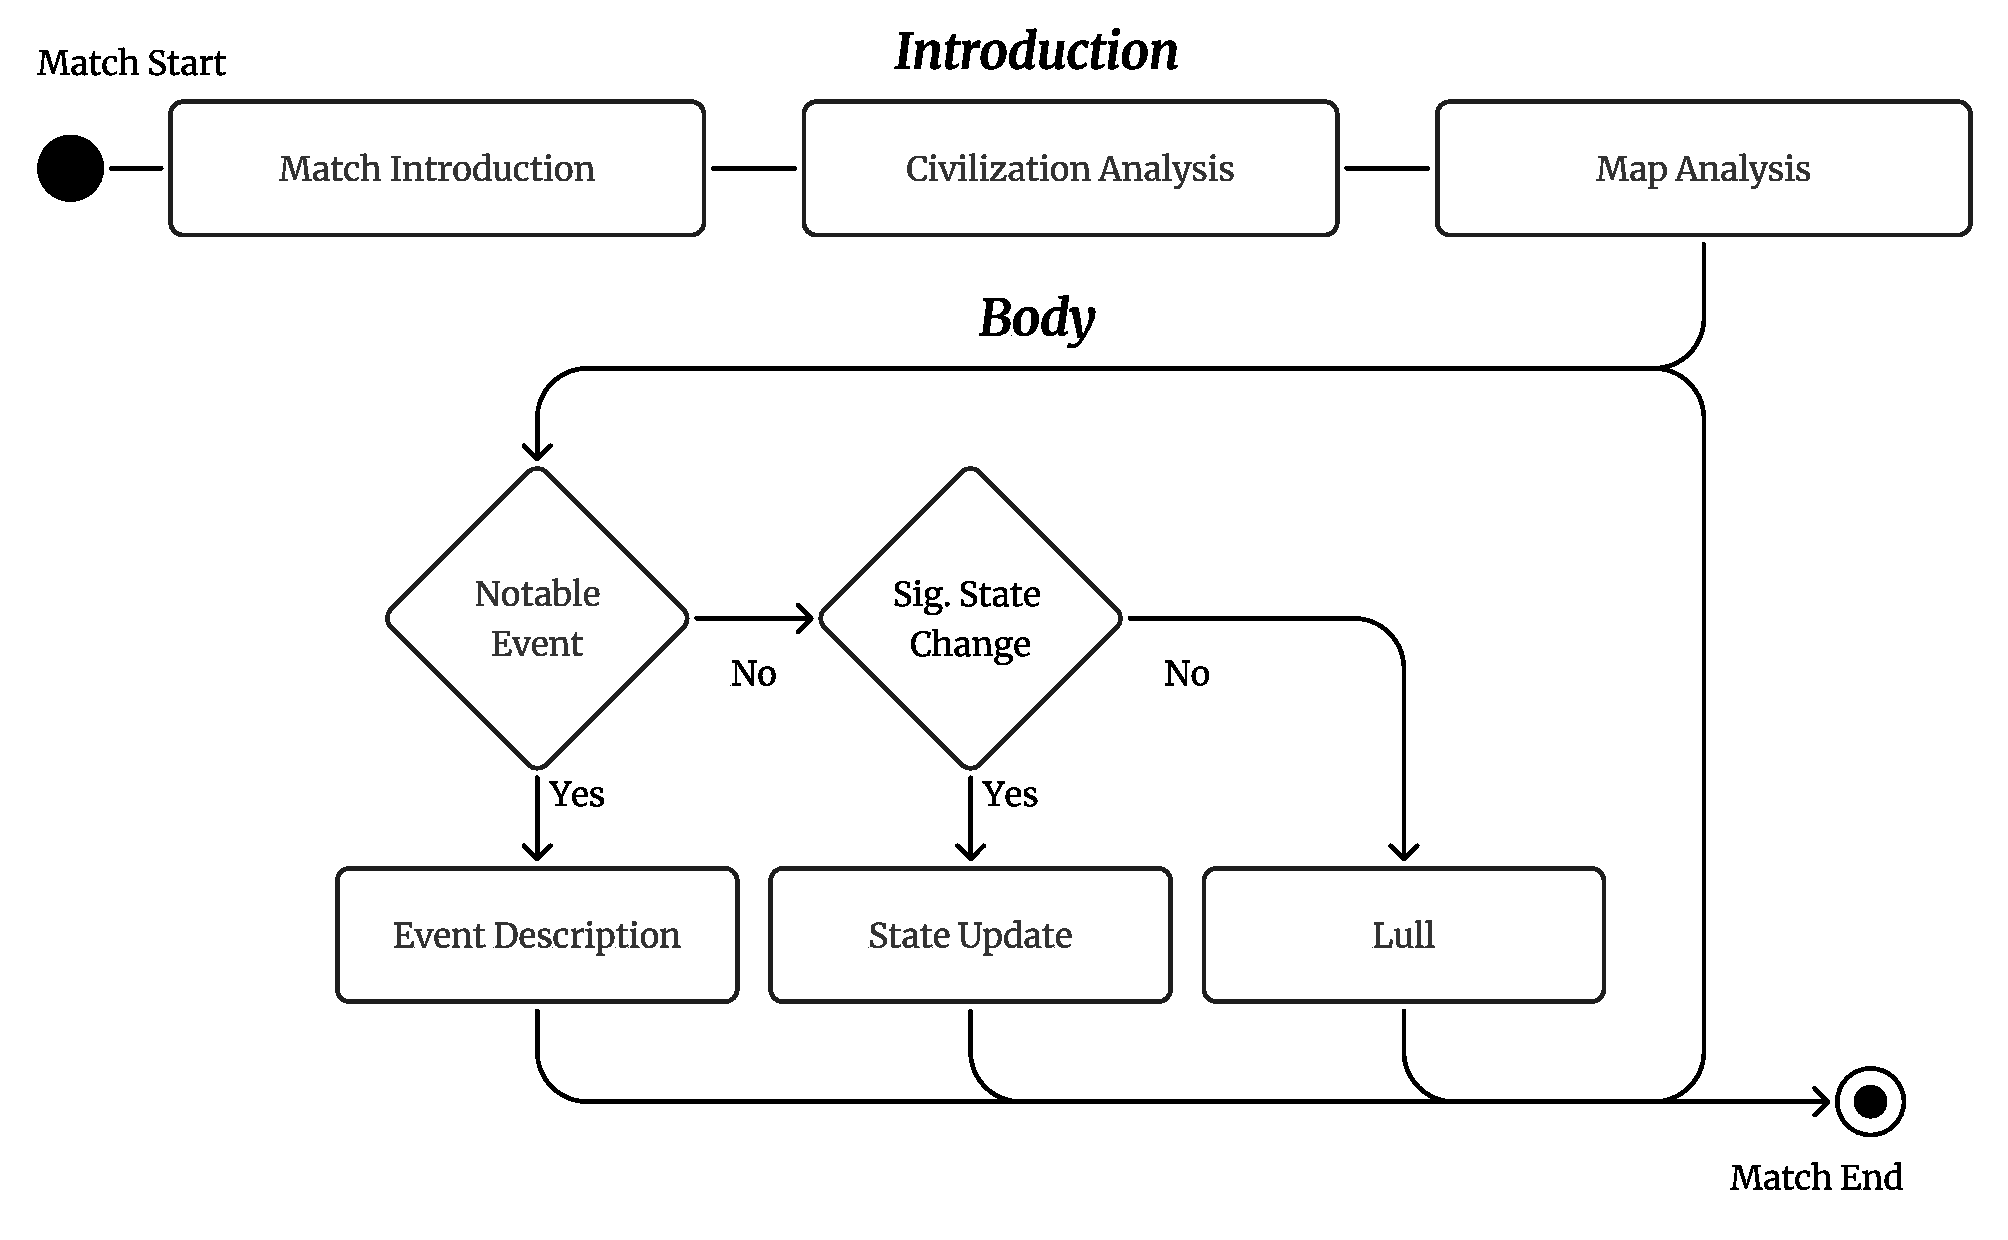
\includegraphics[width=\textwidth]{assets/shoutcasting-structure.pdf}%
  }{%
    \fbox{\parbox{0.95\textwidth}{\centering Placeholder: missing file\\`assets/shoutcasting-structure.pdf`}}%
  }
  \caption{Top-level narrative overview of shoutcasting structure observed across the analyzed casts. It starts with introductions, followed by a loop driven by events, interspersed with state updates and knowledge sharing during lulls.}
  \label{fig:shoutcasting-structure}
\end{figure}

\subsection{Other Observations}
Two recurring themes in the T90 \& Nili cast are consistent with prior findings on esports commentary \cite{lux2019, cheung2011starcraft}. First, T90 \& Nili frequently note the amount of attention points that players need to keep track of and how much is going on, which is in line with \citet{lux2019}'s views on attention points:
\begin{quote}
  \textbf{T90:} \textit{So he’s trying to do a lot right now, and even if he doesn’t want the full wall at this time, he has two idles simply due to how much he’s trying to juggle at the moment.}
\end{quote}
Here Villese is so busy he cannot fully focus on building his wall, leading to idle villagers. This highlights the high cognitive load players are under due to the many attention points they need to keep track of.

Casters also discuss information asymmetry, a key finding of \citet{cheung2011starcraft}. Scouting remarks such as "Does he see it?" highlight cases where casters know more than the player (\textit{Unknown to player, known to caster}):
\begin{quote}
  \textbf{Nili:} \textit{Yeah, that is sometimes the funny situation as a caster, right? We kind of don’t want to lie to our viewers and we kind of want to say, "Okay, what are the next steps to come back?"}\\
  \textbf{Nili:} \textit{Obviously for us, we get the intel, we see everything, we know how bad it looks.}
\end{quote}

This illustrates a common situation: casters see the likely outcome while players lack information. While anecdotal, it suggests these dynamics also hold in AoE2 and are salient to casters.

The other asymmetry types in \citet{cheung2011starcraft} also appear. Players and casters may be uncertain about battle outcomes (\textit{Unknown to player, unknown to caster}):

\begin{quote}
  \textbf{T90:} \textit{Yeah, he should easily clear that, but I think DauT will be happy with how long it took Villese to decide to take that fight, and it wasn’t quite as convincing as I thought it would be either.}
\end{quote}
Here the casters expected a clearer outcome, highlighting uncertainty even for experienced commentators.

Predictions reflect the final asymmetry (\textit{Known to player, unknown to caster}), e.g., forecasting where Villese will place a forward tower.

Because shoutcasts are audiovisual, casters often rely on what viewers see and focus their speech on salient details and transitions, sometimes reflecting only on the beginning and end states of an event.

\section{Discussion}

\subsection{\textbf{RQA1:} How similar is AoE2 to StarCraft II in terms of information and commentary strategies?}
Intelligibility Types (Table~\ref{tab:lim-coding-compare}) and information-foraging patterns (A--E--P+S) closely match SC2 shoutcasting \cite{dodge2018}, confirming that core commentary patterns transfer across RTS titles as an exploratory finding. Because these patterns differ from non-game systems \cite{lim2009}, the similarity appears to reflect RTS/shoutcasting characteristics rather than coincidence, and supports an event-driven prototype grounded in the same frameworks.

\subsection{\textbf{RQA2:} What information and knowledge are used to commentate on these match events?}
Commentary is grounded in \textit{Descriptive} information and enriched with \textit{Domain} and \textit{Analytical} knowledge (Table~\ref{tab:co-occurrence-type-source}). Event Descriptions and State Updates mostly rely on Descriptive information, while Strategy Discussion and Prediction draw more on Domain and Analytical knowledge. For a prototype, this implies detecting actuator-level events (especially battles and key production) and interleaving concise state updates, integrating these layers.

\subsection{\textbf{RQA3:} What narrative structure is used to report on a competitive AoE2 match?}
Figure~\ref{fig:shoutcasting-structure} suggests a recurring event-driven cycle: introductions (match, players, civilizations, map), then cue-driven event reporting enriched with context; lulls are filled with state updates or background knowledge. Two key challenges for an automated system follow:
\begin{enumerate}[noitemsep, topsep=0pt]
  \item Prioritize narratively critical events; frequency is not importance (e.g., a single ``castle drop''---an aggressive forward castle---can outweigh many minor skirmishes).
  \item Handle simultaneous events via summarization or salience selection rather than detailing everything.
\end{enumerate}
These constraints motivate prioritization and concurrency handling (e.g., via summarization or salience selection) in the prototype.

\subsection{Synthesis}
Our AoE2 shoutcasting analysis suggests a cyclical, event-driven pattern: descriptive cues enriched with domain/analytical context. To design a useful system, we must identify which event types and knowledge updates AoE2 viewers value, how to balance action reporting with strategic contextualization, and whether summarization approaches yield coherent narratives. These questions are addressed in the preliminary viewer study (Chapter~\ref{chap:viewer-study}).

\subsection{Limitations}
We did not assess inter-rater reliability as in \citet{dodge2018}: coding was performed by a single coder, and segmentation choices may bias frequencies. We also analyzed only three shoutcasts, limiting generalizability, though the similarity to SC2 suggests the core patterns may transfer within RTS shoutcasting.

Our prototype is text-based, but the analyzed domain is audiovisual: casters rely on what viewers see and may omit details that are visually available. If anything, this may understate Actuator/What content, strengthening the rationale for event-driven summaries.

Finally, we still lack a principled answer to summarization itself: which events matter, and what supporting information is required for a coherent narrative. Event cues interrupt context, but that does not imply contextual information is unimportant. This is best explored through an additional exploratory viewer study, which we conduct in Chapter~\ref{chap:viewer-study}.
